\documentclass[14pt]{extbook}
\usepackage{multicol, enumerate, enumitem, hyperref, color, soul, setspace, parskip, fancyhdr} %General Packages
\usepackage{amssymb, amsthm, amsmath, bbm, latexsym, units, mathtools} %Math Packages
\everymath{\displaystyle} %All math in Display Style
% Packages with additional options
\usepackage[headsep=0.5cm,headheight=12pt, left=1 in,right= 1 in,top= 1 in,bottom= 1 in]{geometry}
\usepackage[usenames,dvipsnames]{xcolor}
\usepackage{dashrule}  % Package to use the command below to create lines between items
\newcommand{\litem}[1]{\item#1\hspace*{-1cm}\rule{\textwidth}{0.4pt}}
\pagestyle{fancy}
\lhead{Makeup Progress Quiz 1}
\chead{}
\rhead{Version B}
\lfoot{6018-3080}
\cfoot{}
\rfoot{Spring 2021}
\begin{document}

\begin{enumerate}
\litem{
Solve the radical equation below. Then, choose the interval(s) that the solution(s) belongs to.\[ \sqrt{9 x + 8} - \sqrt{-3 x - 5} = 0 \]\begin{enumerate}[label=\Alph*.]
\item \( x \in [-0.51,0.28] \)
\item \( \text{All solutions lead to invalid or complex values in the equation.} \)
\item \( x_1 \in [-2.85, -1.53] \text{ and } x_2 \in [-0.89,0.11] \)
\item \( x_1 \in [-1.33, -0.46] \text{ and } x_2 \in [-0.89,0.11] \)
\item \( x \in [-1.33,-0.46] \)

\end{enumerate} }
\litem{
What is the domain of the function below?\[ f(x) = \sqrt[7]{-7 x + 8} \]\begin{enumerate}[label=\Alph*.]
\item \( \text{The domain is } (-\infty, a], \text{   where } a \in [0.64, 1.04] \)
\item \( \text{The domain is } [a, \infty), \text{   where } a \in [1.01, 1.33] \)
\item \( (-\infty, \infty) \)
\item \( \text{The domain is } (-\infty, a], \text{   where } a \in [1.01, 1.23] \)
\item \( \text{The domain is } [a, \infty), \text{   where } a \in [0.78, 0.93] \)

\end{enumerate} }
\litem{
Choose the graph of the equation below.\[ f(x) = - \sqrt[3]{x - 10} + 6 \]\begin{enumerate}[label=\Alph*.]
\begin{multicols}{2}\item 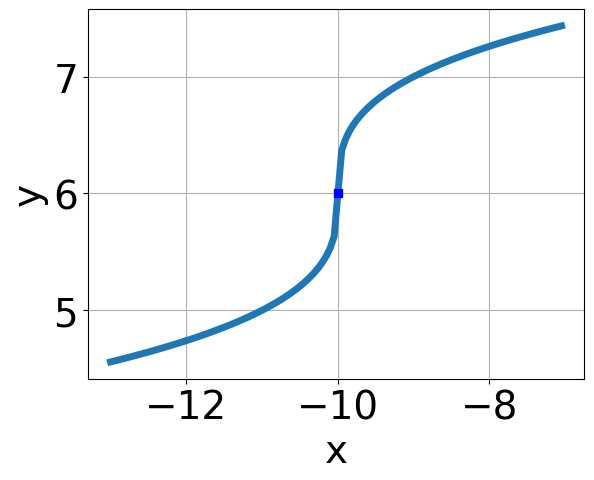
\includegraphics[width = 0.3\textwidth]{../Figures/radicalEquationToGraphAB.png}\item 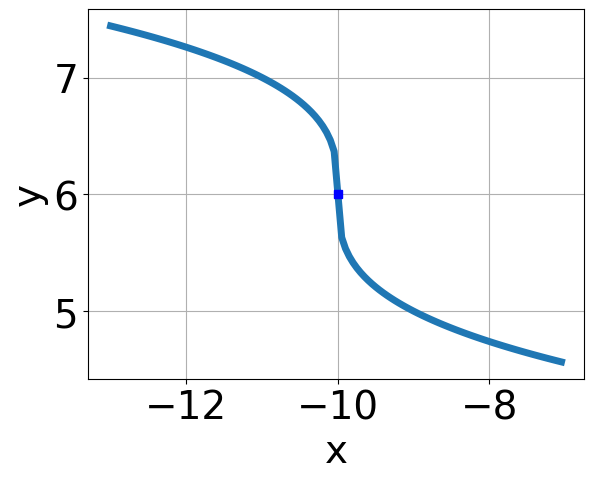
\includegraphics[width = 0.3\textwidth]{../Figures/radicalEquationToGraphBB.png}\item 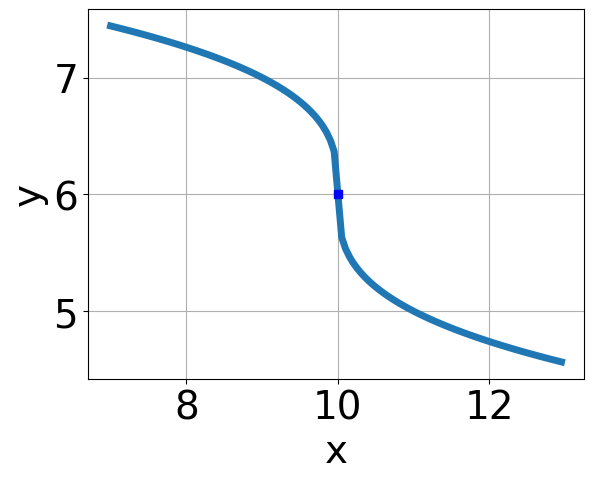
\includegraphics[width = 0.3\textwidth]{../Figures/radicalEquationToGraphCB.png}\item 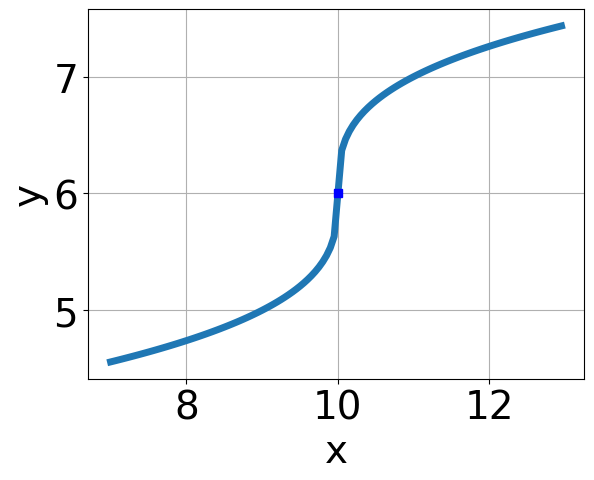
\includegraphics[width = 0.3\textwidth]{../Figures/radicalEquationToGraphDB.png}\end{multicols}\item None of the above.
\end{enumerate} }
\litem{
Solve the radical equation below. Then, choose the interval(s) that the solution(s) belongs to.\[ \sqrt{48 x^2 + 24} - \sqrt{82 x} = 0 \]\begin{enumerate}[label=\Alph*.]
\item \( x \in [0.41,2.23] \)
\item \( x \in [-0.43,0.57] \)
\item \( \text{All solutions lead to invalid or complex values in the equation.} \)
\item \( x_1 \in [-1.63, -0.26] \text{ and } x_2 \in [-0.9,1.1] \)
\item \( x_1 \in [-0.43, 0.57] \text{ and } x_2 \in [1.1,2.1] \)

\end{enumerate} }
\litem{
Choose the equation of the function graphed below.
\begin{center}
    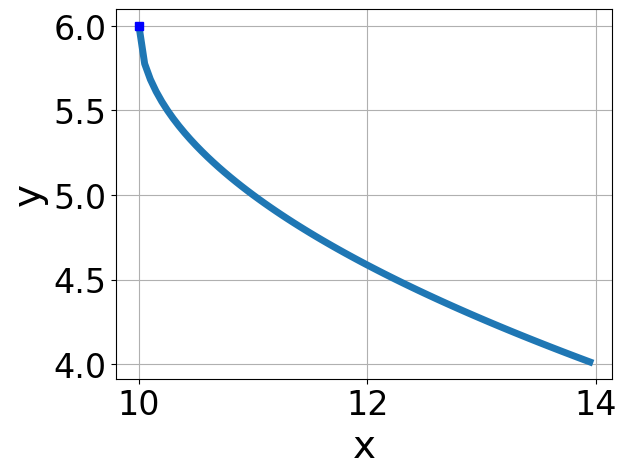
\includegraphics[width=0.5\textwidth]{../Figures/radicalGraphToEquationCopyB.png}
\end{center}
\begin{enumerate}[label=\Alph*.]
\item \( f(x) = - \sqrt[3]{x - 10} + 6 \)
\item \( f(x) = \sqrt[3]{x + 10} + 6 \)
\item \( f(x) = \sqrt[3]{x - 10} + 6 \)
\item \( f(x) = - \sqrt[3]{x + 10} + 6 \)
\item \( \text{None of the above} \)

\end{enumerate} }
\litem{
What is the domain of the function below?\[ f(x) = \sqrt[4]{7 x + 3} \]\begin{enumerate}[label=\Alph*.]
\item \( (-\infty, a], \text{where } a \in [-3, -1.4] \)
\item \( (-\infty, a], \text{where } a \in [-1.7, 0.3] \)
\item \( [a, \infty), \text{ where } a \in [-0.7, 0.7] \)
\item \( [a, \infty), \text{where } a \in [-3.1, -2] \)
\item \( (-\infty, \infty) \)

\end{enumerate} }
\litem{
Solve the radical equation below. Then, choose the interval(s) that the solution(s) belongs to.\[ \sqrt{-36 x^2 - 10} - \sqrt{-53 x} = 0 \]\begin{enumerate}[label=\Alph*.]
\item \( x \in [0.98,1.34] \)
\item \( x \in [0.12,0.27] \)
\item \( \text{All solutions lead to invalid or complex values in the equation.} \)
\item \( x_1 \in [0.12, 0.27] \text{ and } x_2 \in [-0.75,5.25] \)
\item \( x_1 \in [-0.27, -0.16] \text{ and } x_2 \in [-6.25,-0.25] \)

\end{enumerate} }
\litem{
Choose the equation of the function graphed below.
\begin{center}
    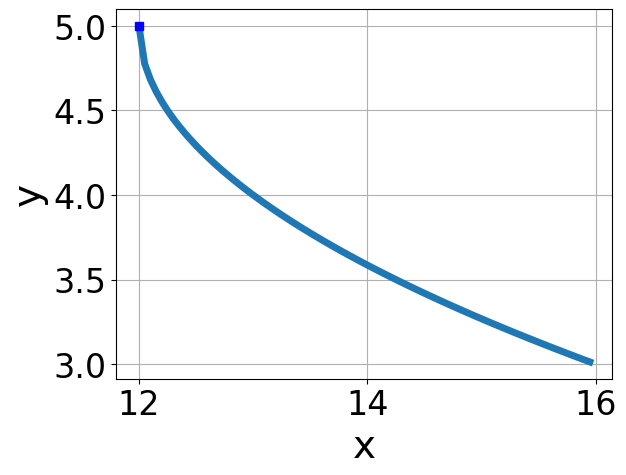
\includegraphics[width=0.5\textwidth]{../Figures/radicalGraphToEquationB.png}
\end{center}
\begin{enumerate}[label=\Alph*.]
\item \( f(x) = - \sqrt[3]{x - 12} + 5 \)
\item \( f(x) = \sqrt[3]{x - 12} + 5 \)
\item \( f(x) = \sqrt[3]{x + 12} + 5 \)
\item \( f(x) = - \sqrt[3]{x + 12} + 5 \)
\item \( \text{None of the above} \)

\end{enumerate} }
\litem{
Solve the radical equation below. Then, choose the interval(s) that the solution(s) belongs to.\[ \sqrt{-7 x + 4} - \sqrt{4 x - 5} = 0 \]\begin{enumerate}[label=\Alph*.]
\item \( \text{All solutions lead to invalid or complex values in the equation.} \)
\item \( x_1 \in [0.23, 0.58] \text{ and } x_2 \in [0.9,2.5] \)
\item \( x \in [-0.15,-0.06] \)
\item \( x_1 \in [0.23, 0.58] \text{ and } x_2 \in [-0.5,1.1] \)
\item \( x \in [0.77,0.89] \)

\end{enumerate} }
\litem{
Choose the graph of the equation below.\[ f(x) = - \sqrt[3]{x - 6} + 5 \]\begin{enumerate}[label=\Alph*.]
\begin{multicols}{2}\item 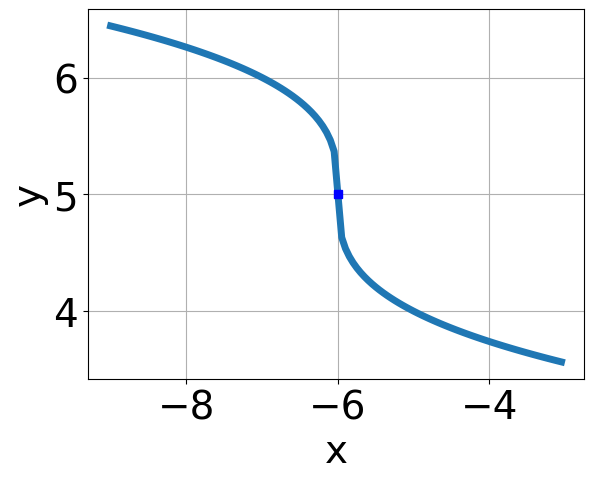
\includegraphics[width = 0.3\textwidth]{../Figures/radicalEquationToGraphCopyAB.png}\item 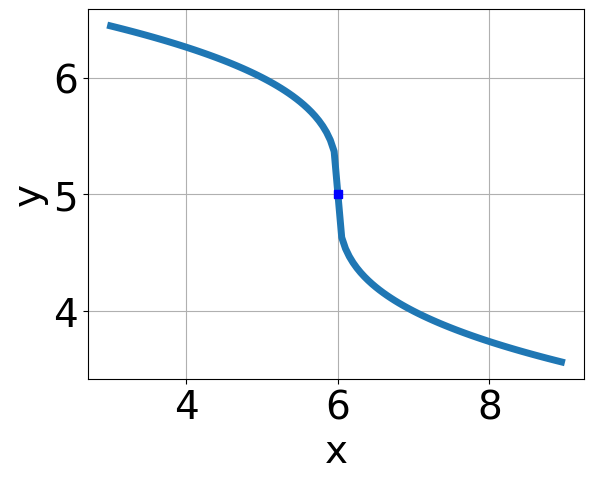
\includegraphics[width = 0.3\textwidth]{../Figures/radicalEquationToGraphCopyBB.png}\item 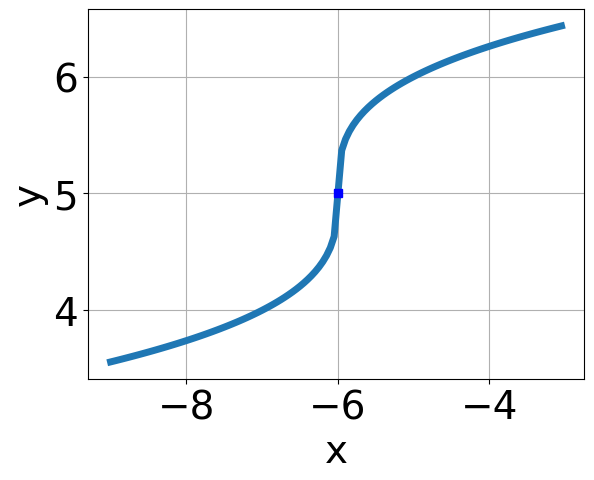
\includegraphics[width = 0.3\textwidth]{../Figures/radicalEquationToGraphCopyCB.png}\item 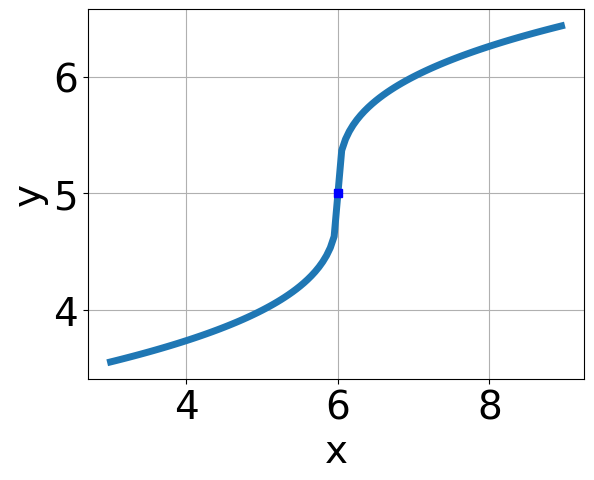
\includegraphics[width = 0.3\textwidth]{../Figures/radicalEquationToGraphCopyDB.png}\end{multicols}\item None of the above.
\end{enumerate} }
\end{enumerate}

\end{document}